\documentclass[professionalfont]{beamer}
\usepackage{newtxtext}
\usepackage[heading = false, scheme = plain]{ctex}
\mode<presentation>{\usetheme{Warsaw}}
\setbeamertemplate{footline}[frame number]
\setbeamertemplate{caption}[numbered]
\usepackage{bbm}
\usepackage{multirow}
\usepackage{amsmath}
\usepackage{listings}
\usepackage{natbib}
\usepackage{xcolor}
\lstset{basicstyle=\tiny\ttfamily,
	numbers=left,
	escapeinside=||
}
\newcommand{\R}[1]{\textcolor{blue}{\small \textrm{#1}}}
\newcommand{\Rout}[1]{\textcolor{green}{\small \textrm{#1}}}
\newcommand{\red}[1]{\textcolor{red}{#1}}
\newcommand{\green}[1]{\textbf{#1}}
\newcommand{\purple}[1]{\textcolor{purple}{#1}}
\newcommand{\blue}[1]{\textcolor{blue}{#1}}
\newcommand{\gray}[1]{\textcolor{gray}{#1}}
\def\bx{\boldsymbol{x}}
\def\bz{\boldsymbol{z}}

\title{第2讲:费率厘定基础~1}
\author{高光远}
\institute{中国人民大学~统计学院}
\date{}
\begin{document}
%%title frame
\begin{frame}
	\titlepage
\end{frame}

\begin{frame}{主要内容}
	\tableofcontents
\end{frame}

%%table of contents
%\AtBeginSection[]
%{
%	\begin{frame}{}
%		\tableofcontents[currentsection]
%	\end{frame}
%}


%%normal frame
\section{风险基础}
	\begin{frame}
	\begin{itemize}
		\item \red{风险基础(exposure base)}是度量\blue{潜在损失大小}的基本工具.
		\item 风险基础也是\blue{保费基础},~决定着\blue{保费(premium)}的高
		低.
		\item \red{风险单位(number of exposures)}是度量风险基础的基本单位,~也称为风险暴露数.
		\end{itemize}	
	\end{frame}
		\begin{frame}{如何选取风险基础?}
		\begin{itemize}
		\item 合理性:风险基础是对潜在损失的准确度量.
		\item 可行性:风险基础便于保险人实际使用和核实.
		\item 客观性:风险基础不易受到人为操纵.
		\item\gray{一致性:和以往的风险基础尽可能一致.}
	    \end{itemize}	
	    
	    ~
	    
	    例:~近年来,~行驶里程数作为风险基础.~如UBI(Usage-based insurance),~PAYD(pay-as-you-drive).
	    
  
		\end{frame}
\subsection{常用的风险基础}
	\begin{frame}
		\begin{itemize}
		\item 机动车交通事故责任强制保险\blue{(交强险)}:~\red{车年}.
		\item {车损险}(\blue{商业车险}):~车年和汽车折旧价.
		\item {第三者责任保险}(\blue{商业车险}):~车年和\red{保险金额}. 保险金额简称\red{保额(amount of insurance, AOI)}.~即保险公司最多赔偿的金额.
		\item \blue{劳工补偿保险(workers' compensation)}:~工资.
	\item 职业责任保险:~保额.
	\item 产品责任保险:~保额.
		\end{itemize}
		
		~
		
		财产保险一般以\green{财产的置换价格}为风险基础;~责任保险一般以\green{保额}为风险基础.
	\end{frame}

\subsection{风险单位统计量}
	\begin{frame}{}
		\begin{enumerate}
	\item \blue{承保}风险单位数(\blue{written} exposures):~不论是否到期;~若有中途退保,~承保风险单位数为\green{负}.
	\item \blue{到期}风险单位数(\blue{earned} exposures):~已经承担的风险单位数.
	\item \blue{未到期}风险单位数(\blue{unearned} exposures):~未承担的风险单位数.
	\item \blue{有效}风险单位数(\blue{in-force} exposures):~在\green{某一时刻}所有未到期的保单的承保风险单位数.

		\end{enumerate}
	
	~
	
	1,2建立在\green{时间段}上;~3,4建立在\green{时间点}上.
	\end{frame}
\begin{frame}
	\begin{table}[]
		\centering
		\caption{保险期限为一年的三份汽车保单}
		\label{my-label}
		\begin{tabular}{ccccccc}
			\hline
			\multirow{2}{*}{保单} & \multirow{2}{*}{生效日期} & \multicolumn{2}{c}{承保风险} & \multicolumn{2}{c}{到期风险} & 有效风险     \\ \cline{3-7} 
			&                       & 2004       & 2005        & 2004        & 2005       & 2005/1/1 \\ \hline
			1                   & 2004/1/1              & 1          & 0           & 1           & 0          & 0        \\
			2                   & 2004/4/1              & 1          & 0           & 0.75        & 0.25       & 1        \\
			$3^*$               & 2004/7/1              & 1          &\green{-0.25}       & 0.5         & 0.25       & 1        \\
			& 合计                    & 3          & -0.25       & 2.25        & 0.5        & 2        \\ \hline
			\multicolumn{7}{l}{*:保单3在2005/4/1退保.}                                               \\ \hline
		\end{tabular}
	\end{table}
\end{frame}	



\section{保费}
\begin{frame}
	\begin{center}
\red{保费=赔款+理赔费用+承保费用+利润附加}

~

\red{Premium=Loss payment + Loss adjustment expense + Underwriting expense + Profit loading}
	\end{center}
	
\end{frame}
\subsection{赔款}
\begin{frame}{赔款}
\begin{itemize}
	\item \red{赔款(claims payment, loss payment)}是保险公司根据\blue{保险合同}的约定支付给\blue{索赔人(claimant)}的款项.~赔款是\blue{随机变量(random variable)}.
	\item \gray{赔款可以分为两部分:~已付赔款和未决赔款.~其中未决赔款包括:~个案准备金,~已发生未完全报案赔款和已发生未报案赔款.~这部分内容在未决赔款准备金评估中有详细的描述.}
	\item \red{期望赔付成本}是赔款的\blue{期望(expectation)}.

	
\end{itemize}	
\end{frame}
\begin{frame}{索赔频率(claim frequency)和索赔强度(claim severity)}

	\begin{itemize}
	\item 风险模型课程主要研究了:\blue{索赔次数}的分布 (如Poisson,negative binomial等),~\blue{索赔金额}的分布 (如log-normal,gamma等) 和它们的复合分布 (如compound Poisson-gamma).
	\item \red{索赔频率(claim frequency)}是指在一定时期内\green{平均}每个风险单位的索赔次数.
	\item \red{索赔强度(claim severity)}是指\green{平均}每次索赔的金额.

	
	\end{itemize}
\end{frame}
\begin{frame}{回归模型(regression models)}
	\begin{itemize}
\item  风险模型课程中没有引入\blue{协变量(自变量,covariates,features)}.
\item \blue{分类费率厘定}(以后详细讲)将引入\red{风险因子(risk factors)}作为协变量,建立\blue{回归模型(regression models)}对索赔频率和索赔强度进行预测.
\item 
常用的索赔频率(次数)模型为\green{泊松回归模型}:
$$N_i\sim \text{Poi}(\nu_i\lambda_i);~\lambda_i=f(\bx_i)$$
其中$N_i$为第$i$辆车的索赔次数,~$\nu_i$为车年数,~$\lambda_i$为索赔频率,~$\bx_i$为风险因子.

\item 常用的索赔强度(金额)模型为\green{伽马回归模型}:
$$Y_i\sim \text{Gam}(\zeta_i,\phi);~\zeta_i=g(\bz_i)$$
其中$Y_i$为第$i$辆车的索赔金额,~$\zeta_i$为索赔强度,~$\phi$为\blue{离散系数(dispersion)},~$\bz_i$为风险因子.
	\end{itemize}
\end{frame}	
\begin{frame}
	\begin{itemize}
	\item 为什么对索赔频率与强度分别建模,~而不直接对赔款$N_iY_i$建模?\pause \\ \green{影响$\lambda_i$和$\zeta_i$的风险因子不同;~即$\bx_i\neq\bz_i$. }\pause
	\item 对于某一保单,~是否可以直接对\green{截止到某一时刻}的索赔次数和索赔金额建立模型?\pause\\\green{不可以,~这些数字没有真实地反应该保单的实际(最终)赔付.}~\green{判断是否为最终索赔次数时需要考虑}\red{报案延迟(report delay)},~\green{判断是否为最终赔款金额时需要考虑}\red{报案延迟}\green{和}\red{赔付延迟(payment delay)}.
	\end{itemize}
\end{frame}

\subsection{费用和利润附加}
\begin{frame}
	\begin{itemize}
		\item \red{承保费用(underwriting expenses).}~在卖出和管理保险合同时发生的费用,~包括:~代理人佣金,~一般管理费用,~广告费,~税金等.
		\item \red{理赔费用(loss adjustment expenses,LAE).}~在结案过程中发生的费用,~包括:~\blue{直接理赔费用(allocated LAE, ALAE)和间接理赔费用(unallocated LAE, ULAE).}
		\item 盈利是保险公司经营保险产品的一个重要目的.
	\end{itemize}
\end{frame}
\begin{frame}
	\begin{figure}
		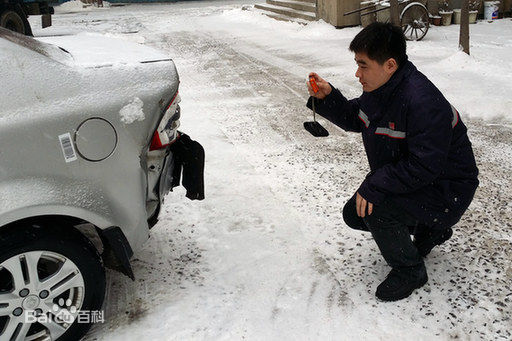
\includegraphics[width=0.45\textwidth]{Plots/ALAE.jpg}~~
		
\includegraphics[width=0.45\textwidth]{Plots/ULAE.jpg}
		\caption{ALAE and ULAE}
	\end{figure}
\end{frame}
\subsection{纯费率}
\begin{frame}
~ ~ ~\red{纯费率(pure premium)}\\=\green{单位风险}的期望赔付成本\\
=最终赔款/风险单位数\\=(最终赔款/赔款次数)$\times$(赔款次数/风险单位数)\\=索赔频率$\lambda_i\times$索赔强度$\zeta_i.$

~

\begin{itemize}
	\item 纯费率厘定关键是对索赔频率和索赔强度建立回归模型. 
	\item 传统的回归模型包\blue{括线性回归(linear models),~广义线性模型(generalized linear models,GLM),~广义可加模型(generalized additive models,GAM)}.~ 这些模型要求知道回归方程$f,g$的形式.
	\item \blue{监督机器学习(supervised machine learning),~如decision tree, neural network},~不需要知道回归方程$f,g$的形式.
	\item 纯费率厘定是(初级)精算师的一个核心工作,另一个核心工作是准备金评估(后面会讲到).
\end{itemize}


\end{frame}
\subsection{保费统计量}
\begin{frame}
类似于风险单位统计量,~有以下的保费统计量\\

~

\begin{itemize}
	\item 承保保费(written premium)
	\item 已赚保费(earned premium)
	\item 未赚保费(unearned premium)
\end{itemize}

~

在计算已赚保费(已赚风险单位数)和未赚保费(未赚风险单位数)时,~一个隐含假设是\green{风险在时间轴上均匀分布.}

\end{frame}

\section{赔付率等}
\subsection{赔付率}
\begin{frame}
	\red{赔付率(loss ratio)}是指每单位保费中用于支付赔款的部分,~通常用赔款与保费之比进行估计.
	
	~
	
	\begin{itemize}
		\item 严格地讲,~为了实现保费和赔款之间的配比关系,~应该用\blue{最终赔款(ultimate loss,ultimate claims)}与已赚保费.
		\item 有时把理赔费用也包含在赔款中,~这时称为\blue{赔款和理赔费用比率(loss and LAE ratio)}.
		\item 在费率厘定中,~最常用的比率就是赔付率.
	\end{itemize}
\end{frame}
\subsection{其它比率}
\begin{frame}
	\begin{itemize}
		\item \blue{理赔费用比率(loss adjustment expense ratio)}:~理赔费用和\green{赔款}之比.
		\item \blue{承保费用比率(underwriting expense ratio)}:~承保费用和\green{保费}之比.
		\begin{enumerate}
			\item 发生在保单\green{签发时}的费用与\green{承保}保费相比.~如代理人佣金,~广告费,~税金等.
			\item 发生在保单\green{期间}的费用与\green{已赚}保费相比.~如一般管理费.
			\item 把以上两部分比率相加得到承保费用比率.
		\end{enumerate}
		\end{itemize}
\end{frame}
\begin{frame}
	\begin{itemize}
		\item \blue{经营费用比率(operational expense ratio)}:~费用和保费之比.~由以下两部分组成:
		\begin{enumerate}
			\item 理赔费用与已赚保费之比
			\item 承保费用比率
		\end{enumerate}
		\item \red{综合成本率(combined ratio)}:~赔款和费用在保费中的比例.~是\green{衡量保险业务利润水平}的主要指标.~由以下三部分组成:
		\begin{enumerate}
			\item 赔付率
			\item 理赔费用与已赚保费之比
			\item 承保费用比率
		\end{enumerate}
	\end{itemize}
\end{frame}
\begin{frame}
	\begin{itemize}
		\item \blue{续保率(retation ratio)}:~实际续保保单数和潜在可续保保单数之比.
		\item \blue{签约率(conversion ratio)}:~实际签订合同的人数和收到公司报价的人数之比.
	\end{itemize}
\end{frame}
\begin{frame}
	\begin{figure}
		
\includegraphics[width=0.45\textwidth]{Plots/retation.jpg}
		\caption{续保率}
	\end{figure}
\end{frame}
\section{费率手册和网页报价}
\begin{frame}
	\blue{费率手册(ratemaking manual,rating plan)}是保险公司对风险进行分类并计算其保费的一种文件.~通常包括:~费率表(rating tables),~定价公式(rating algorithm),~使用说明.~在实际应用中,~费率手册通常需要与承保指南(under writing guideline)配合使用.
	
	~
	
	在信息技术未成熟前,~精算师负责制定费率手册;~目前,~大部分车险都可以网页报价.
\end{frame}
\begin{frame}
	\begin{figure}
		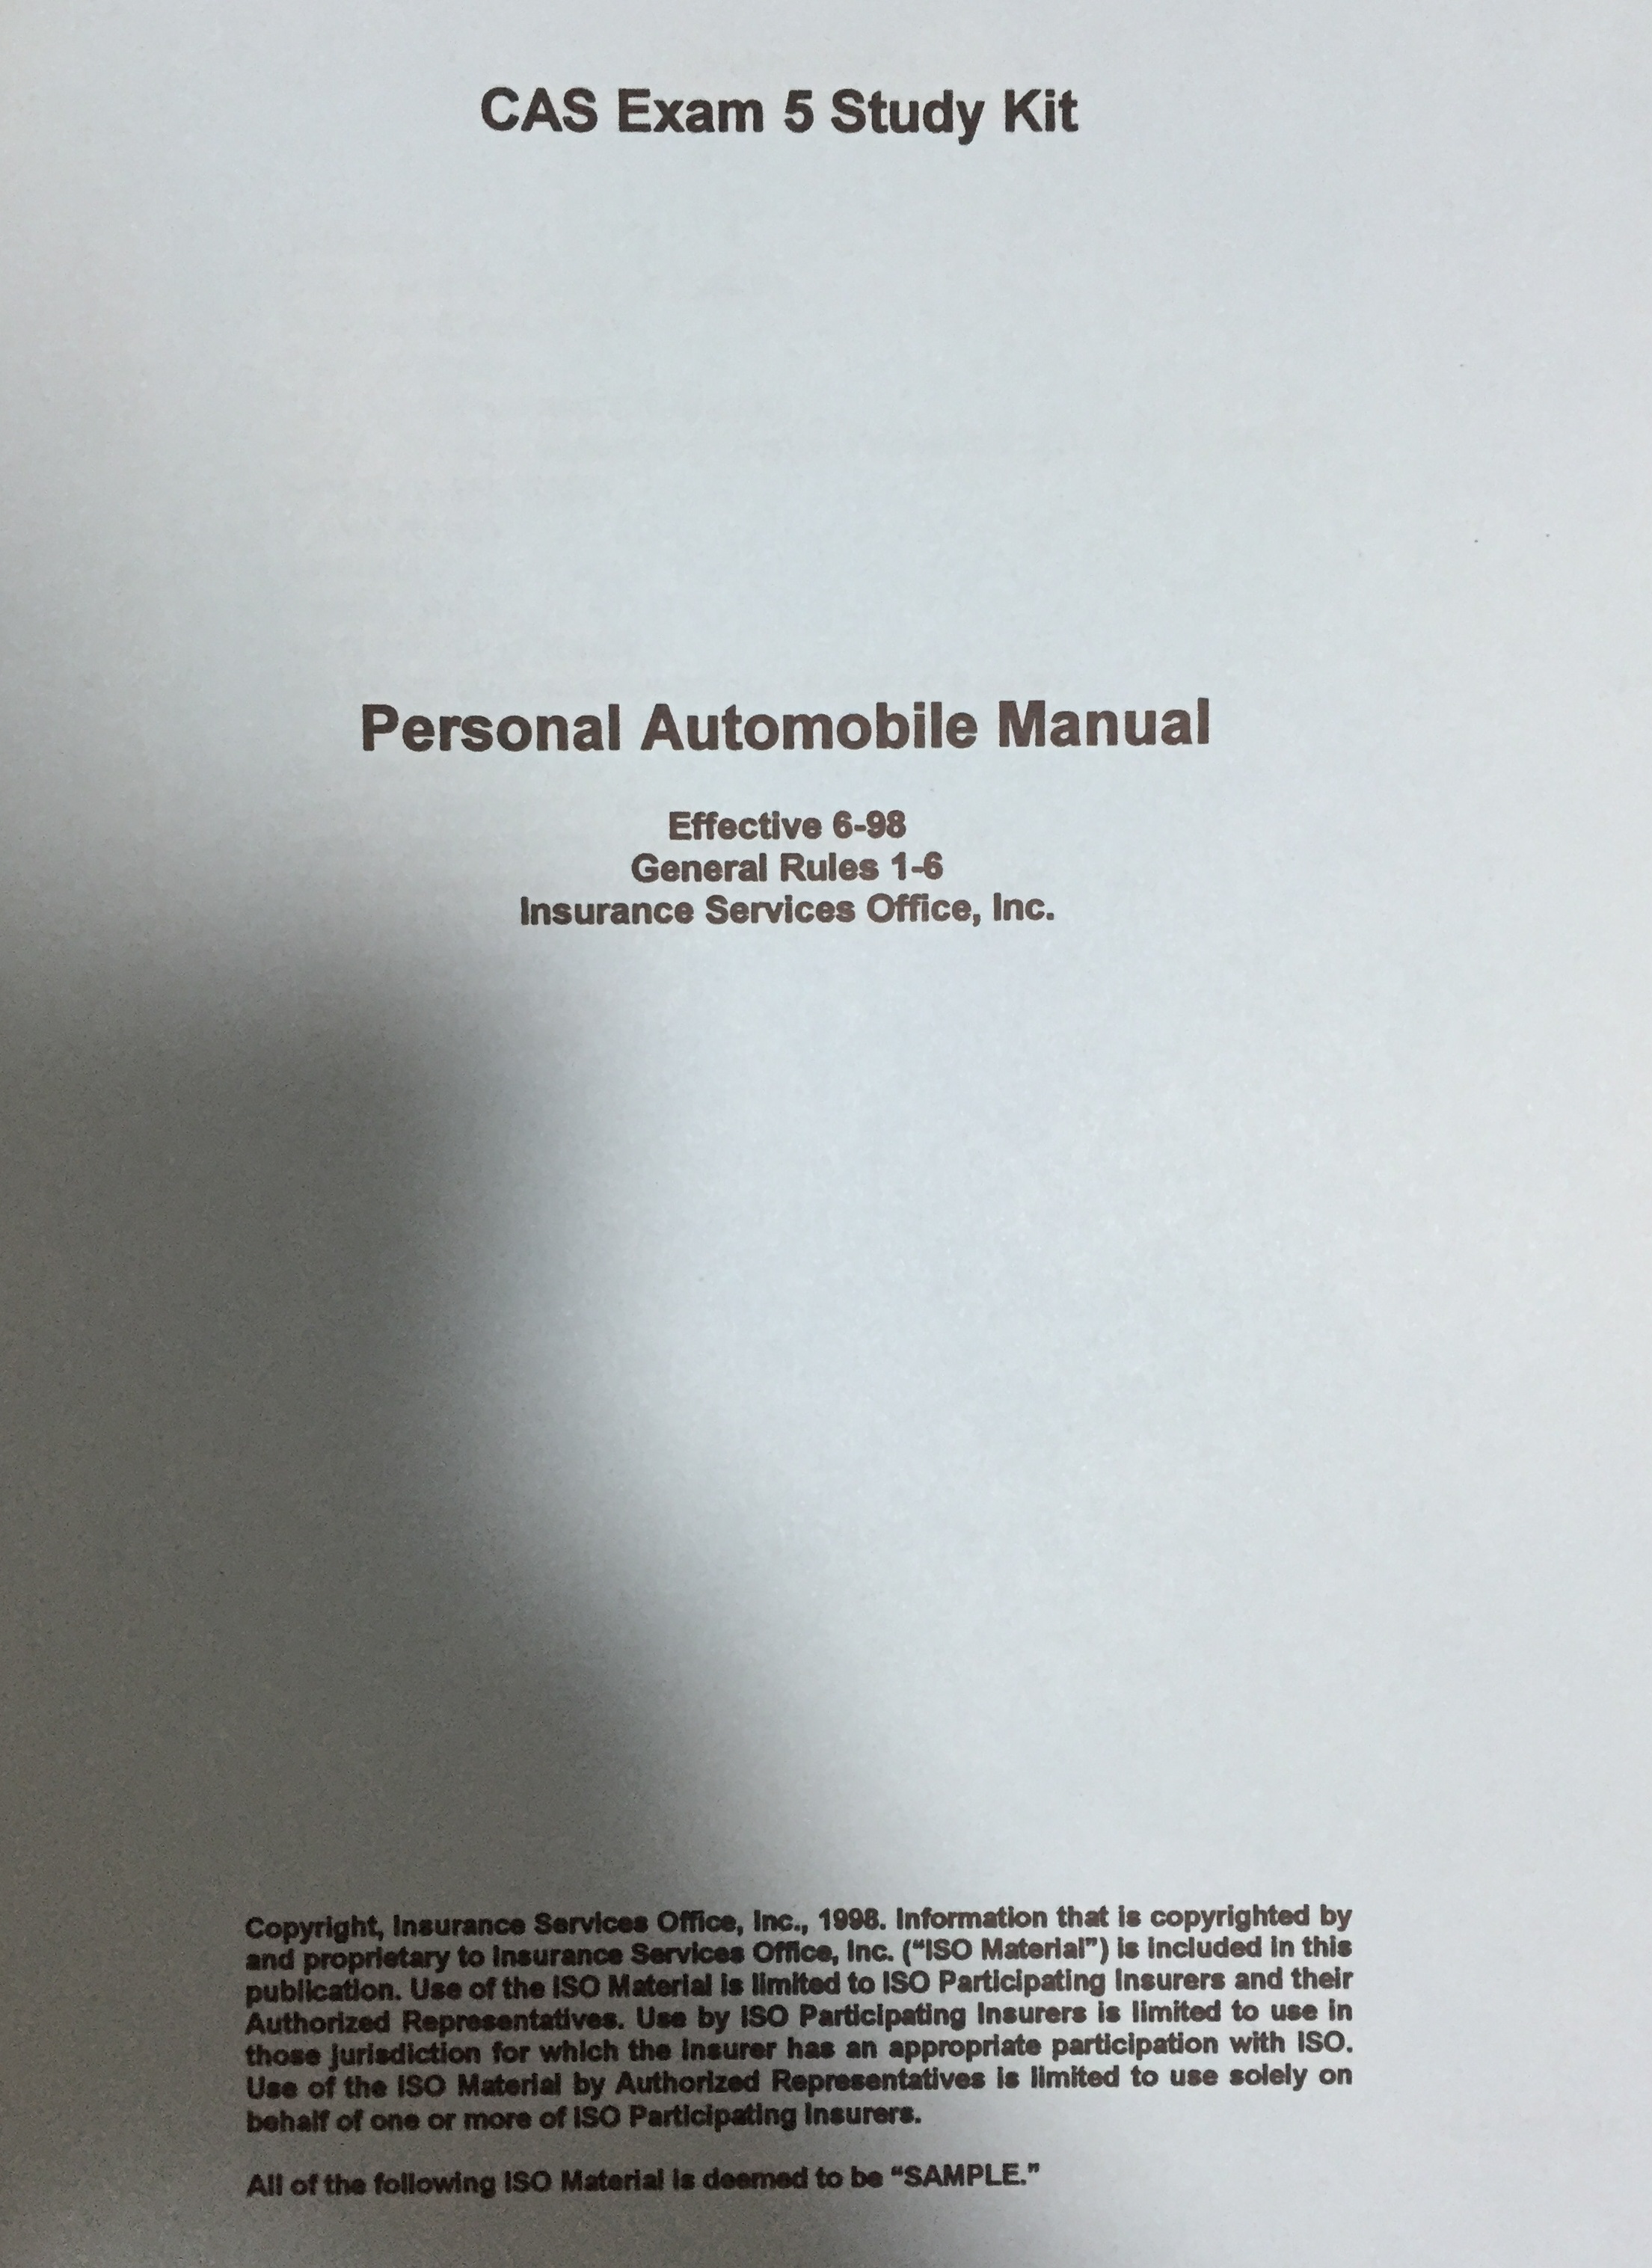
\includegraphics[height=0.45\textwidth]{Plots/manual1.jpg} ~~
		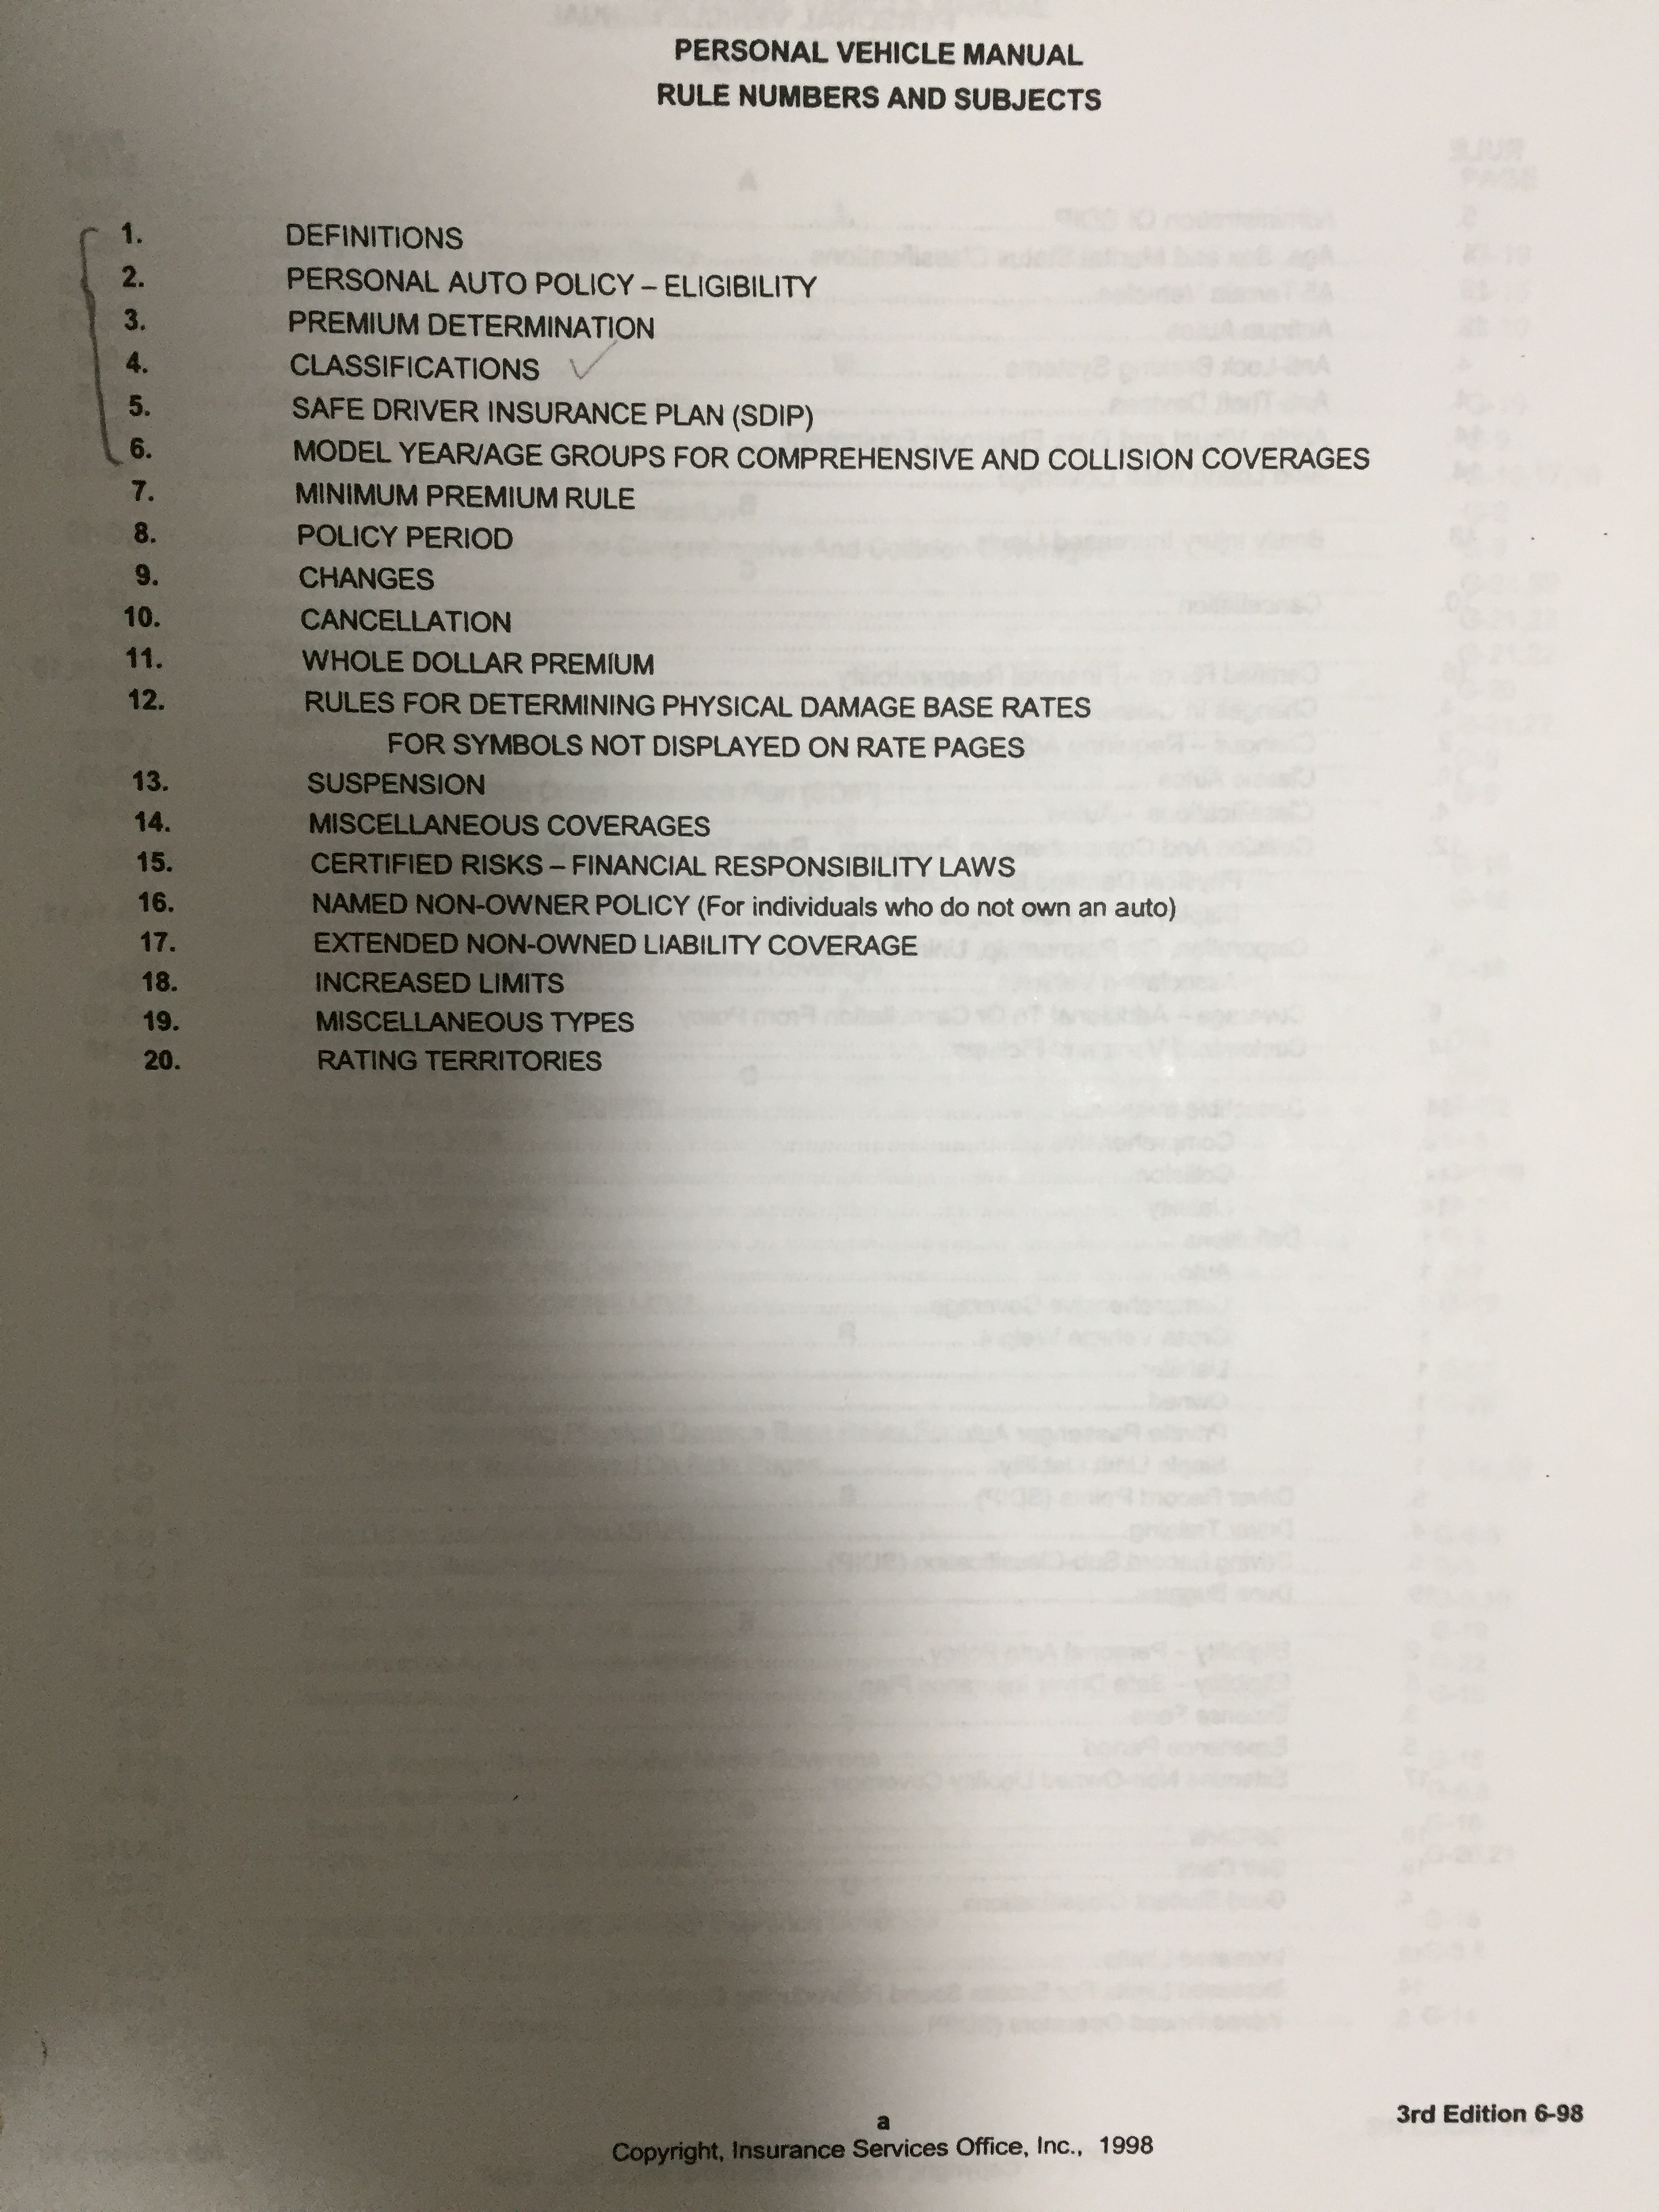
\includegraphics[height=0.45\textwidth]{Plots/manual2.jpg}
		\caption{费率手册}
	\end{figure}
\end{frame}
\begin{frame}
		\begin{figure}
			
\includegraphics[width=\textwidth]{Plots/website_price.png}
			\caption{网页报价}
		\end{figure}
\end{frame}
\section*{}
\begin{frame}
	\begin{enumerate}
		 \item  阅读教材3.1.
		 \item 自测课后练习题.
		 \item 欢迎通过邮箱nonlife\_actuarial@163.com提问.
		\item 总成绩100=课堂60+期末40.
		\item 其中,课堂=作业90+表现10.
	\end{enumerate}
\end{frame}


\end{document}